% Document setup
\documentclass[11pt]{book}

% Location of the csas-style repository: adjust path as needed
\newcommand{\locRepo}{csas-style}

% Use the style file in the csas-style repository (sr.sty)
\usepackage{\locRepo/sr}

% header-includes from R markdown entry


% Bibliography style file
% \bibliographystyle{../csas-style/res-doc}

%%%% Commands for title page etc %%%%%

% Title
\newcommand{\rdTitle}{STOCK STATUS UPDATE OF AMERICAN LOBSTER (\emph{HOMARUS AMERICANUS}) IN LOBSTER FISHING AREA 41 (4X + 5ZC)}

% French title
\newcommand{\rdTitleFr}{Titre Ici (\emph{Nom Latin})}

% Title short
\newcommand{\rdTitleShort}{Short Title}

% Publication year
\newcommand{\rdYear}{20XX}

% Publication month
\newcommand{\rdMonth}{January}

% Report number
\newcommand{\rdNumber}{nnn}

% Approver (name\\position)
\newcommand{\rdApp}{Approver Name\\
Regional Director}
% \newcommand{\rdYear}{20XX}
% \newcommand{\rdAppMonth}{January}
% \newcommand{\rdAppDay}{1}
\newcommand{\rdAppDate}{January 1, 20XX}

% Branch
\newcommand{\rdBranch}{Science Branch}

% Region
\newcommand{\rdRegion}{Pacific Region}

% Address
\newcommand{\rdAddress}{\textsuperscript{1}Pacific Biological Station\\
Fisheries and Oceans Canada, 3190 Hammond Bay Road\\
Nanaimo, British Columbia, V9T 6N7, Canada\\
\textsuperscript{2}Far, far away\\
Another Galaxy}

% Phone
\newcommand{\rdPhone}{(250) 756-7208}

% Email
\newcommand{\rdEmail}{\href{mailto:csap@dfo-mpo.gc.ca}{\nolinkurl{csap@dfo-mpo.gc.ca}}}

%%%% End of title page commands %%%%%
\begin{document}

\bookmark[dest=PageOne]{\rdTitle{}}

\MakeFirstPage

\hypertarget{context}{%
\section{Context}\label{context}}

The status of Lobster in Lobster Fishing Area (LFA) 41 was last assessed in the fall of 2017 (DFO 2018; Cook et al.~2017) with annual updates in the following years. This update applies the suite of indicators from the 2017 assessment to the stock status up to the end of the 2020 season (wherever possible). Indicators for Lobster in LFA 41 are consistent with the Department of Fisheries and Oceans (DFO) precautionary approach and allow for the evaluation and monitoring of the offshore Lobster. This Science Response Report results from the Science Response Process of October 22, 2020, on the Stock Status Update of American Lobster in Lobster Fishing Area (LFA) 41.

\hypertarget{background}{%
\section{Background}\label{background}}

Commercial Lobster fishing in LFA 41 (Figure 1) occurs offshore, from the 50 nautical mile line (92 km) to the upper continental slope, within Northwest Atlantic Fisheries Organization (NAFO) Divisions 4X and 5Zc. The areal extent of the LFA extends to the easterly extent of the 4V NAFO line.

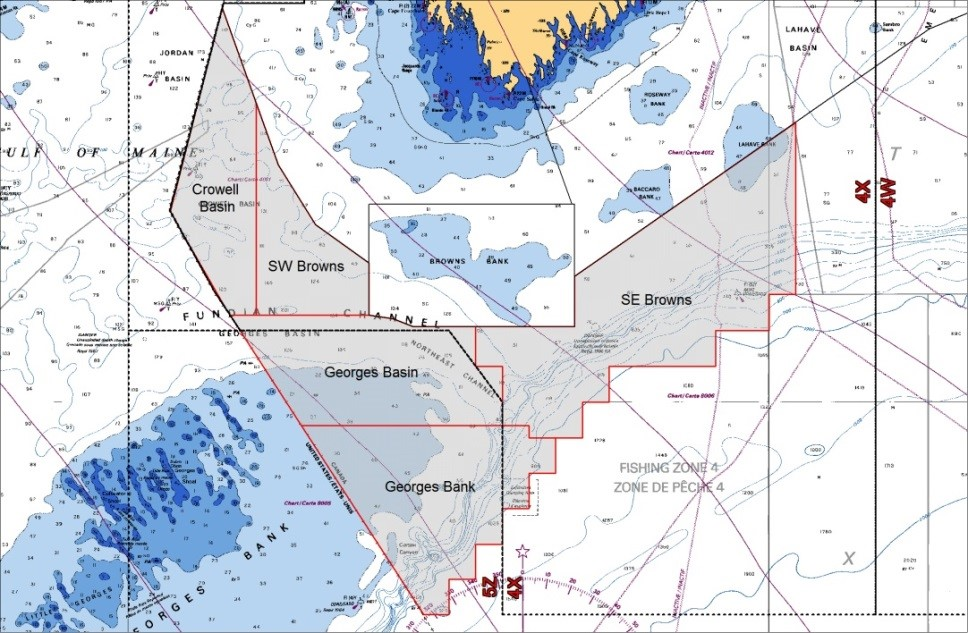
\includegraphics{C:/Users/Howsevj/Documents/LFA41_UpdateMD/41map.jpg}

Figure 1: Map showing LFA 41 offshore subareas for primary indicators (4X -- Crowell Basin, Southwest Browns, and Southeast Browns, and 5Z -- Georges Basin and Georges Bank).

The LFA 41 fishery operates under the Offshore Lobster and Jonah Crab Integrated Fisheries Management Plan. It is the only Lobster fishery in Canada that is managed under a Total Allowable Catch (TAC). The minimum legal size is 82.5 mm carapace length, and there is a prohibition on landing berried and v-notched females. The fishery operates year round. Currently, there is no trap limit.

The annual TAC (720 t) was established in 1985 based on historical landings. Annual landings from 2002 to 2019 are presented in Figure 2. In recent years, the TAC has been managed under a three-year management cycle that allows for quota overruns and carry-forward of uncaught quota. At the end of the third year of a cycle, no more than three times the annual quotas (i.e., no more than 2,160 t) may be landed.
\begin{figure}[htb]

{\centering \pdftooltip{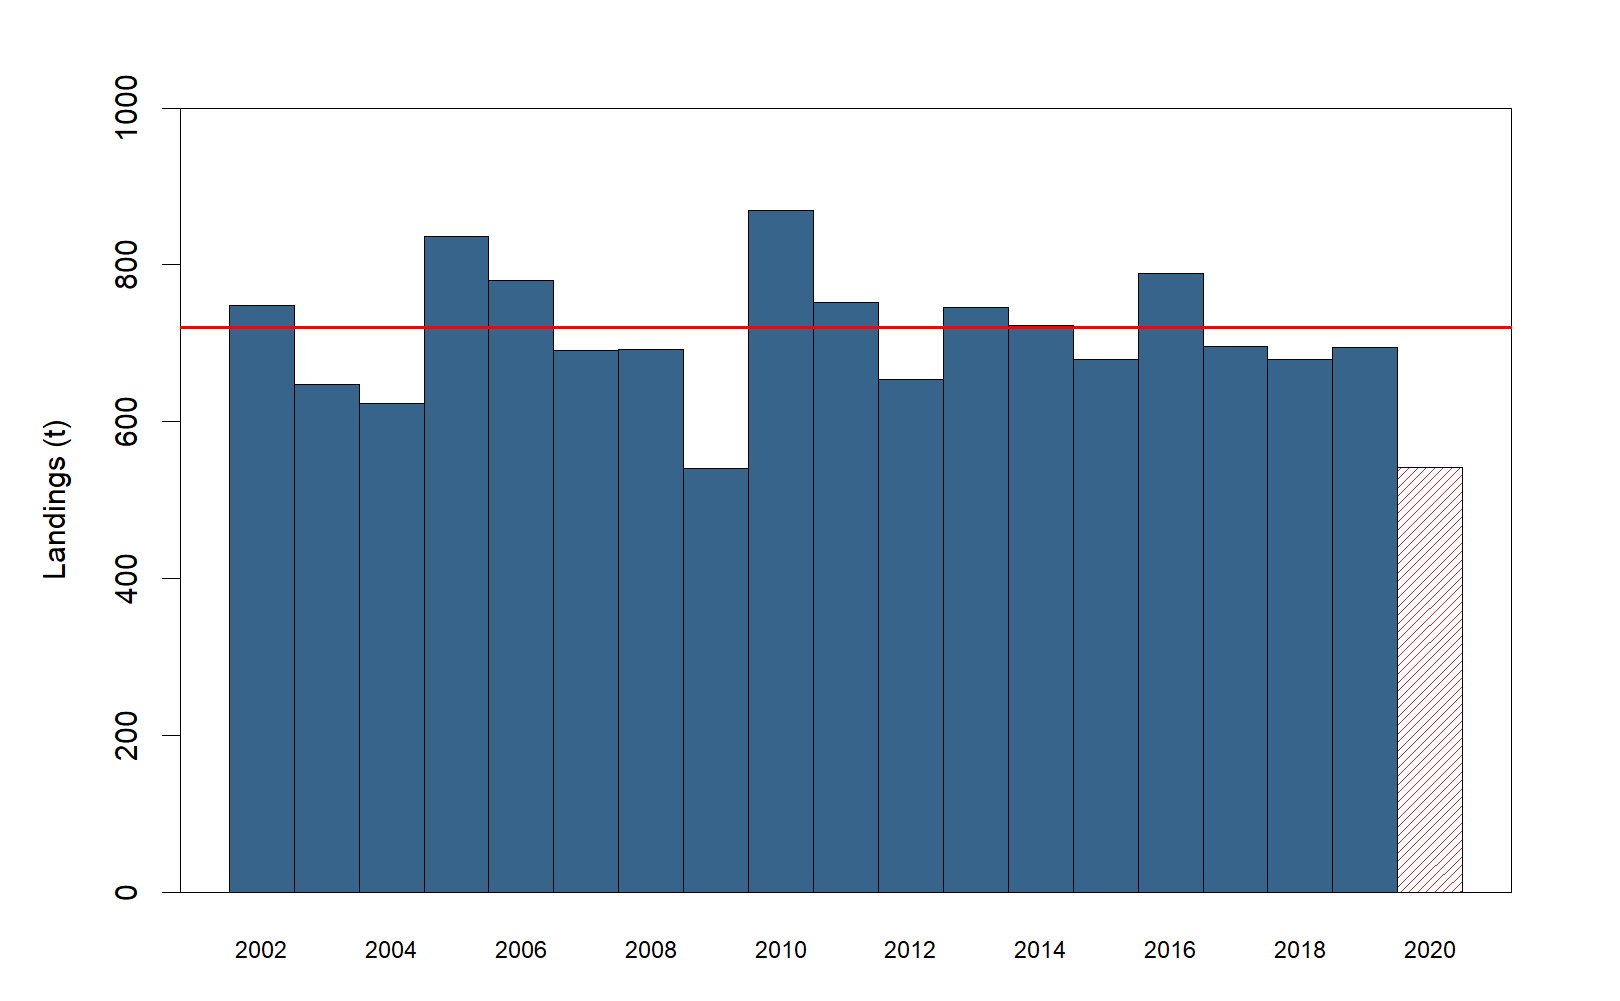
\includegraphics[width=6in]{knitr-figs-pdf/landings-1}}{Figure} 

}

\caption{Landings (t) for Lobster Fishing Area 41 from 2002-2020 against a Total Allowable Catch of 720t. Horizontal red line denotes the TAC. Note: Red bar (hash marks) for 2020 landings indicates data is incomplete.}\label{fig:landings}
\end{figure}
\hypertarget{analysis-and-response}{%
\subsection{Analysis and Response}\label{analysis-and-response}}

\hypertarget{indicators-of-stock-status}{%
\subsubsection{Indicators of Stock Status}\label{indicators-of-stock-status}}

The status of Lobster in LFA 41 is assessed using two indicators of stock health: survey commercial biomass and reproductive potential. The reference points defining the Healthy, Cautious and Critical zones -- the Upper Stock Reference (USR) and the Limit Reference Point (LRP) -- are based on the survey biomass. Both indicators use fishery independent data available from four multispecies surveys, two conducted by DFO and two conducted by the Northeast Fisheries Science Centre (NEFSC). The DFO Summer Research Vessel Survey (RV41) covers the offshore portions on the Scotian Shelf, and the DFO Spring Research Vessel Survey (GB) covers the offshore portions on Georges Bank. The NEFSC surveys cover the Gulf of Maine and Georges Bank in the spring (NSpr41) and autumn (Naut41).

\hypertarget{primary-indicators-and-stock-status}{%
\subsubsection{Primary Indicators and Stock Status}\label{primary-indicators-and-stock-status}}

\hypertarget{commercial-biomass-from-research-vessel-surveys}{%
\subsubsection{Commercial Biomass from Research Vessel Surveys}\label{commercial-biomass-from-research-vessel-surveys}}

Lobster biomass is measured by four multispecies surveys from which commercial biomass indices are used to determine overall stock health. The commercial biomass is calculated for each survey, and a three-year running median is used to assess stock status relative to reference indicators. The Limit Reference Indicator (LRI) for each index is defined as the median of the five lowest non-zero biomasses in the time series. The Upper Stock Indicator (USI) is defined as 40\% of the median of the higher productivity period (i.e., 2000--2015). For the stock to be considered in the Healthy Zone, the commercial biomass indices for at least three of the four surveys must be above their respective USIs (Figure 3). Currently, all four surveys are above their respective USIs. Therefore, the stock is considered to be in the Healthy Zone, and it has been since 2002.
\begin{figure}[htb]

{\centering \pdftooltip{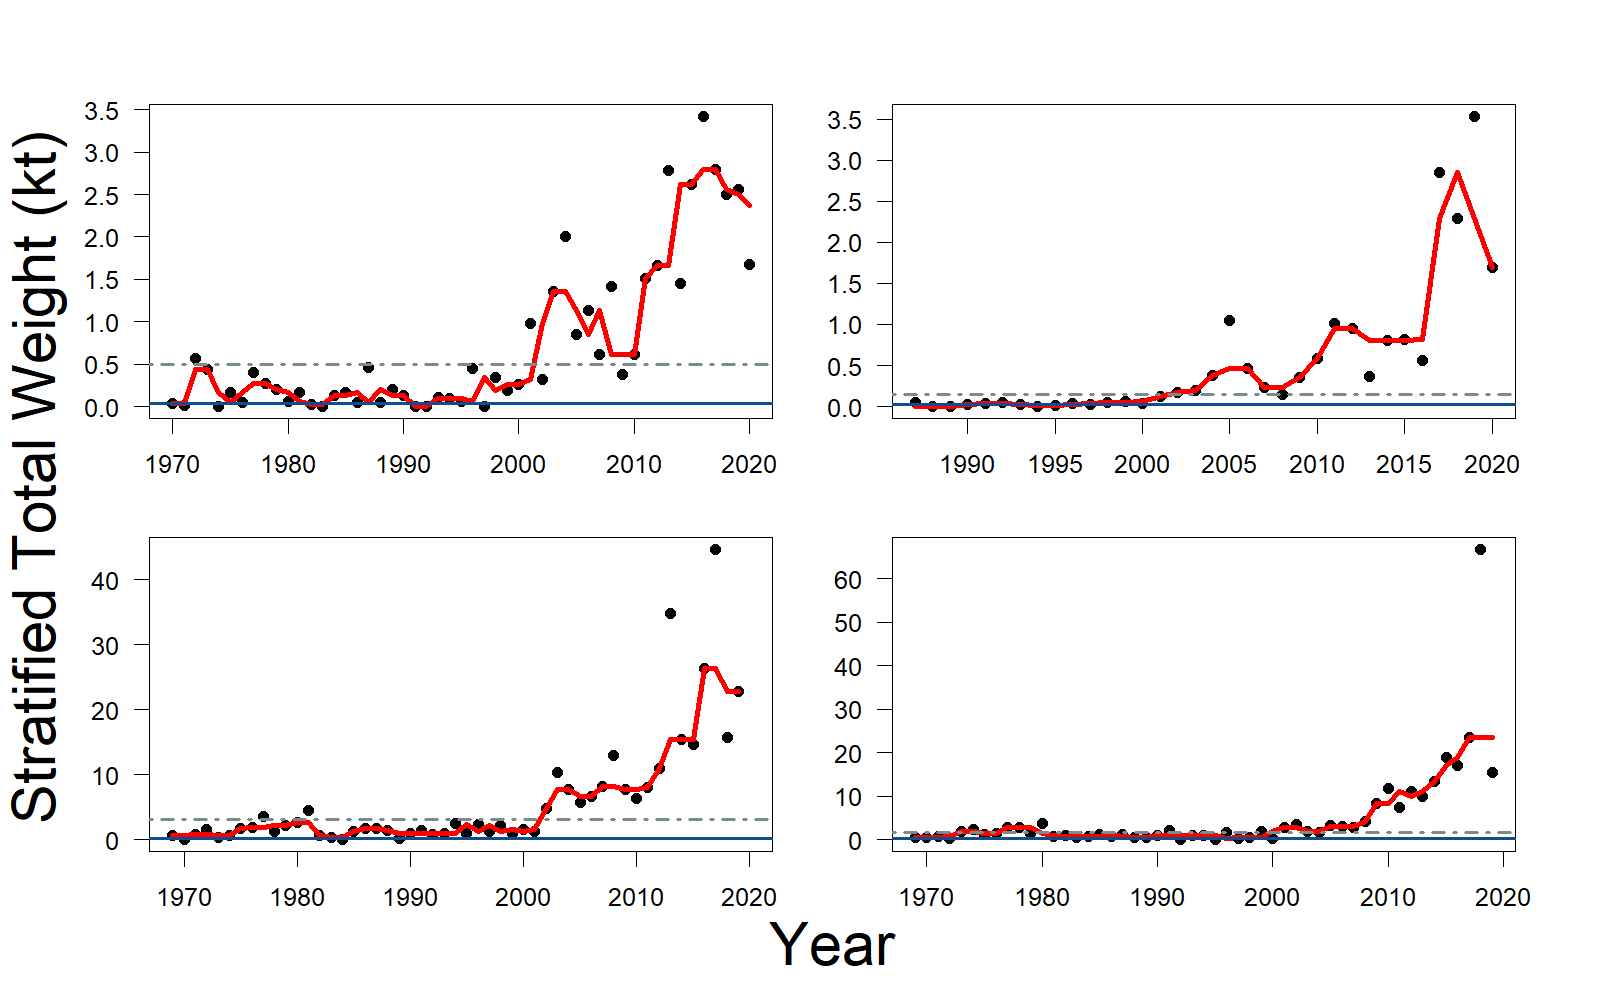
\includegraphics[width=6in]{knitr-figs-pdf/Primary biomass-1}}{Figure} 

}

\caption{ Commercial biomass time series along with the 3-year running median (red line), compared to LRI (solid blue line), and  USI (dot-dash grey line). Top row: left- RV41, right – GB. Bottom row: left –NSpr41, right – Naut41. Note: Different scales used on both x-axis and y-axis.}(\#fig:Primary biomass)
\end{figure}
\hypertarget{reproductive-potential}{%
\subsubsection{Reproductive Potential}\label{reproductive-potential}}

Reproductive potential consists of an integrated index combining female abundance at size, fecundity at size, and size-at-maturity. It represents an estimate of total eggs produced within the stock area and can also be viewed as a surrogate for Spawning Stock Biomass (SSB). An Upper Boundary (UB) and Lower Boundary (LB) have been set (where sufficient data is available) to help gauge the significance of changes in egg production relative to long-term medians. Reproductive potential is above the long-term median and the respective UBs in all survey indices. Estimates of reproductive potential are at or near the highest values on record (Figure 4). An increase in overall abundance was the main driver of the increase in reproductive potential despite a decrease in median size of the Lobsters as was observed in the at-sea samples and documented during the 2017 stock assessment.
\begin{verbatim}
FALSE png 
FALSE   2
\end{verbatim}
\#\#\#Bycatch

At-sea observer data is aggregated by three-year time blocks to represent average annual bycatch estimates in LFA 41 (Table 1). Bycatch amounts for crabs (Cancer), Cusk, and Atlantic Cod have decreased consistently since 2009. Non-retained Lobster catch consists of undersized, berried, v-notched and potentially cull (one or zero claws), soft and jumbos (≥ 140 mm Carapace Length {[}CL{]}). The target for observed trips is 6 per season for LFA 41. The total number of trips, observed trips, and the percent of observer coverage are reported in Table 2.

\hypertarget{conclusions}{%
\section{Conclusions}\label{conclusions}}

The primary indicators of stock status for Lobster in LFA 41 show the stock is in the Healthy Zone, with all four multispecies survey commercial biomass indices above their respective USIs. Reproductive potential estimates were also above the upper boundaries where defined. Despite not having a removal reference or estimates of removal rates, the TAC of 720 t poses minimal risk to the stock status falling into the Cautious Zone, as the stock has proven its resilience to this level of removal.

\hypertarget{contributors}{%
\section{Contributors}\label{contributors}}

Mandatory section and title.
\begin{longtable}[]{@{}ll@{}}
\toprule
Name & Affiliation\tabularnewline
\midrule
\endhead
Victoria Howse & DFO Science, Maritimes Region\tabularnewline
Adam Cook & DFO Science, Maritimes Region\tabularnewline
Cheryl Denton & DFO Science, Maritimes Region\tabularnewline
Verna Docherty & DFO Fisheries Management , Maritimes Region\tabularnewline
Rabindra Singh & DFO Science, Maritimes Region\tabularnewline
Brad Hubley & DFO Science, Maritimes Region\tabularnewline
Kyle Gillespie & DFO Science, Maritimes Region\tabularnewline
\bottomrule
\end{longtable}
\MakeApproval

\hypertarget{sources-of-information}{%
\section{Sources of information}\label{sources-of-information}}

Cook, A.M., Cassista Da-Ros, M., and Denton, C. 2017. Framework Assessment of the Offshore American Lobster (Homarus americanus) in Lobster Fishing Area (LFA) 41. DFO Can. Sci. Advis. Sec. Res. Doc. 2017/065. viii + 186 p.

DFO. 2018. Assessment of Lobster (Homarus americanus) in Lobster Fishing Area 41 (4X + 5Z) for 2016. DFO Can. Sci. Advis. Sec. Sci. Advis. Rep.~2018/004.

\MakeAvailable

\end{document}
